\section{Observations}

\begin{frame}{The Substitution box}
\begin{itemize}
    \item In the original version of the cipher (KHAZAD-0) tabular replacement was represented by a classic S-block.
    \item In the modified version of the cipher, the S-block 8x8 is modified and represented by a recursive structure consisting of mini-blocks P and Q
    \item Each of which is a small replacement block with 4 bits at the input and output (4x4).
\end{itemize}
\end{frame}

\begin{frame}{The Substitution box}
\begin{itemize}
    \item Recursive structure of the replacement unit in the modified KHAZAD cipher: \\
\begin{center}
    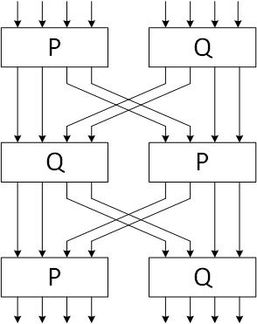
\includegraphics[scale=0.3]{Screenshots/RecStructure.jpg}
\end{center} 

\item This structure of P and Q-mini blocks is equivalent to the S-block with the following substitution table:
\begin{center}
    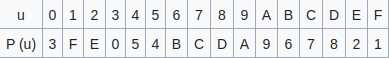
\includegraphics[scale=0.5]{Screenshots/ps1.png}
\end{center}
\begin{center}
    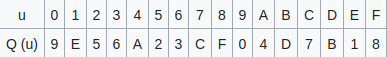
\includegraphics[scale=0.5]{Screenshots/qs1.png}
\end{center}
\end{itemize}
\end{frame}

\begin{frame}{S-box}
\begin{center}
    \textbf{The final KHAZAD S-box}\\
    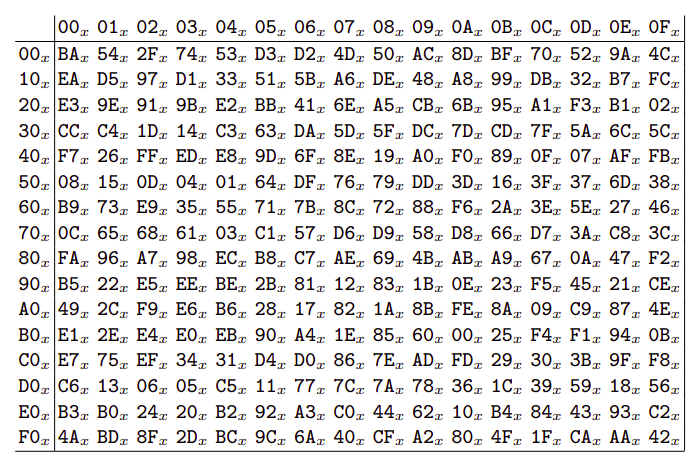
\includegraphics[scale=0.4]{Screenshots/sbox.png}    
\end{center}
\end{frame}


\begin{frame}{Attacks on Khazad}
\begin{enumerate}
    \item Khazad belong to group of ciphers which consists of Shark, Square, Rijndael, Anubis.
    \item These were made in such a way that
     differential attack and linear attacks are not successful attacks for them.
     \item It is very unusual to be successful for these ciphers on their full versions.
\end{enumerate}
\end{frame}

\begin{frame}{Differential attack}
\begin{enumerate}
    \item A differential attack exists for a 3 rounds Khazad cipher but its time complexity is very large as compared to 3 round integral attack.
    \item Lets see the effect of each round on the message block due to different layers.
\end{enumerate}
\end{frame}

\begin{frame}{The 3 round differential attack}
    \begin{center}
        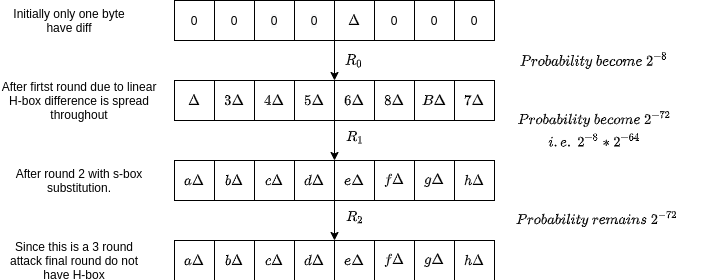
\includegraphics[scale=0.47]{Screenshots/diffat.png}
    \end{center}
\end{frame}

\begin{frame}{The 3 round differential attack}
\begin{center}
    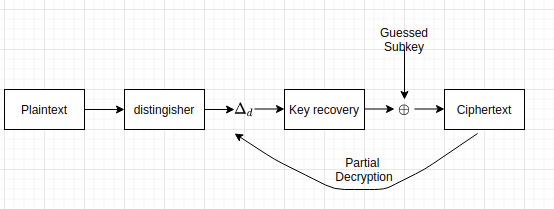
\includegraphics[scale=0.45]{Screenshots/pd.png}
\end{center}
So after guessing 8 bytes of key or guessing subkey there would be at max $2^{64}$ possible guesses for 8 bytes of subkey, therefore the time complexity achieved would be $2^{64}$
\begin{table}[h]
\centering
\begin{tabular}{|l|l|l|}
\hline
Attack Type     & Rounds & Time     \\ \hline
differential attack & 3      & $2^{64}$  \\ \hline
\end{tabular}
\end{table} 
\end{frame}


\begin{frame}{DDT}
    The DDT for s-box of KHAZAD can be created similar to how it was created for other block ciphers.
    \begin{center}
    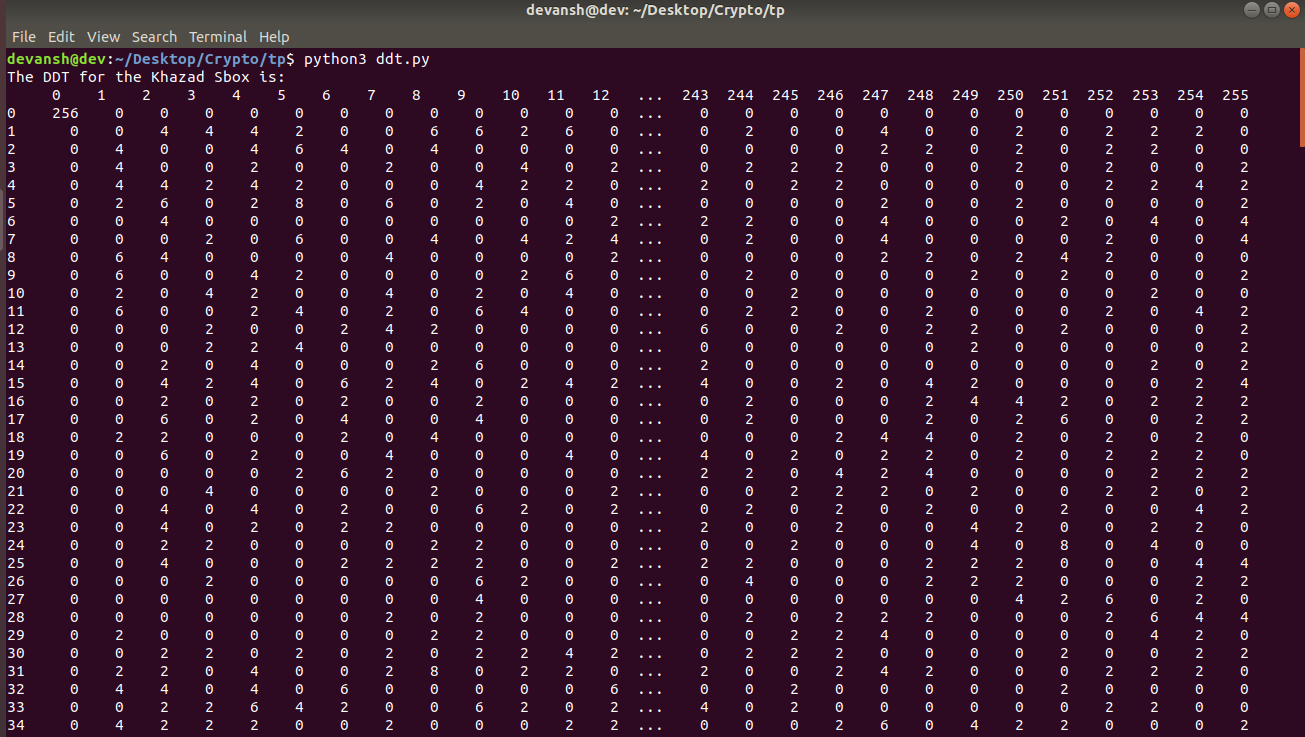
\includegraphics[scale=0.14]{Screenshots/k_ddt.png}\\
\end{center}
There were around 100 s-box transitions like 5 - 5 ,  4 - 2E,  7 - 86  having the best probability equal to $\frac{8}{16} = 0.5$. Any of the byte can be taken accordingly for differential attack.
\end{frame}

\begin{frame}{Integral attack}
Also known as the \textbf{The Square Attack}. The integral attack consists of the following properties.
The attack is set on a
256 plaintexts, such that the first byte takes all 256 possible values
while other bytes have constant values.
\begin{itemize}
    \item \textbf{The All property: }The All property is the byte in which all values come once among the texts in the set.It is denoted by \textit{\textbf{A}}.
    \item \textbf{The Constant property: }The constant property refers to the byte in which all texts in the set have the same value. It is denoted by \textit{\textbf{C}}.
    \item \textbf{The Balanced property : }Also called the 0-sum property, the balanced property refers to the byte in which sum of all the texts in the set is 0.It is denoted by \textit{\textbf{B}}.
\end{itemize}
\end{frame}

\begin{frame}{The 3 round integral attack}
    \begin{center}
    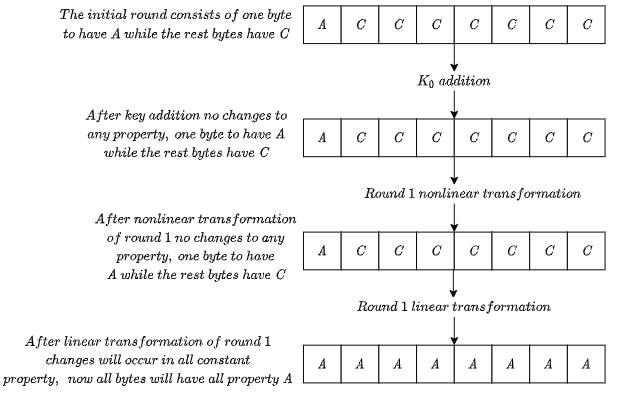
\includegraphics[scale=0.5]{Screenshots/r01.png}  
\end{center} 
\end{frame}

\begin{frame}{The 3 round integral attack}
    \begin{center}
    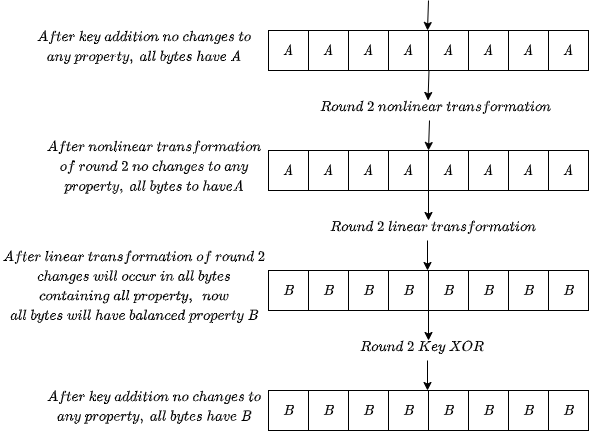
\includegraphics[scale=0.5]{Screenshots/r12.png}  
\end{center} 
\end{frame}

\begin{frame}{The 3 round integral attack}
\begin{enumerate}
    \item All bytes in our plaintexts will have balanced property after 2 rounds.
    \item No H-box or linear transformation in the last round.
    \item sub-key guessed separately to do a complete 3-rounds attack here.
    \item The complexity of this attack will be nearly $2^{16}$ sbox looks and $2^9$ plaintexts selections. Also we can increase this attack to 4 rounds by guessing the other subkey and this will increase time complexity by $2^{64}$.
    \item The 3 round integral attack's complexity is:
\end{enumerate}
\begin{table}[h]
\centering
\begin{tabular}{|l|l|l|l|}
\hline
Attack Type     & Rounds & Time     & Space \\ \hline
integral attack-1 & 3      & $2^{16}$ & $2^9$ \\ \hline
\end{tabular}
\end{table}
\end{frame}

\begin{frame}{The 4 round integral attack and beyond}
    The another variant is 4 round integral attack where we guess the other subkey.
\begin{table}[h]
\centering
\begin{tabular}{|l|l|l|l|}
\hline
Attack Type     & Rounds & Time     & Space \\ \hline
integral attack-2 & 4      & $2^{80}$ & $2^9$ \\ \hline
\end{tabular}
\end{table}
\begin{itemize}
    \item Improved Integral attack for 5 rounds.
    \item Weak Keys Attack
    \item Interpolation attack
    \item The boomerang attack
\end{itemize}
\end{frame}
